\section*{Introduction}
\label{s:Introduction}
API documentation is an essential part of the software development process, it
improves the dev experience and makes it easier to integrate, improves
maintainability and conveniently enables versioning with indication on
deprecated fields \citep{fanWhyAPIDocumentation2021}. Working with API
documentation is not always straightforward, especially when working with
gateway and federation, as it would require much effort from all the developers
involved in the process. Swagger makes documentation for REST-APIs very
straightforward, as it automatically generates HTML based visualisation and
interaction out of the box for any consumer of the API
\citep{korenExploitationOpenAPIDocumentation2018}. Since Facebook released
GraphQL to the mass in 2015, many individual developers and companies are
switching and converting to it to build their APIs, as it enables them to have a
much more flexible and efficient way of building their APIs
\citep{britoRESTVsGraphQL2020}. GraphQL gives to the consumer only the data that
he needs, solving the overfetching and underfetching problem related to the
traditional REST-APIs \citep{witternGeneratingGraphQLWrappersREST2018}.
\begin{figure}[H]
  \centering
  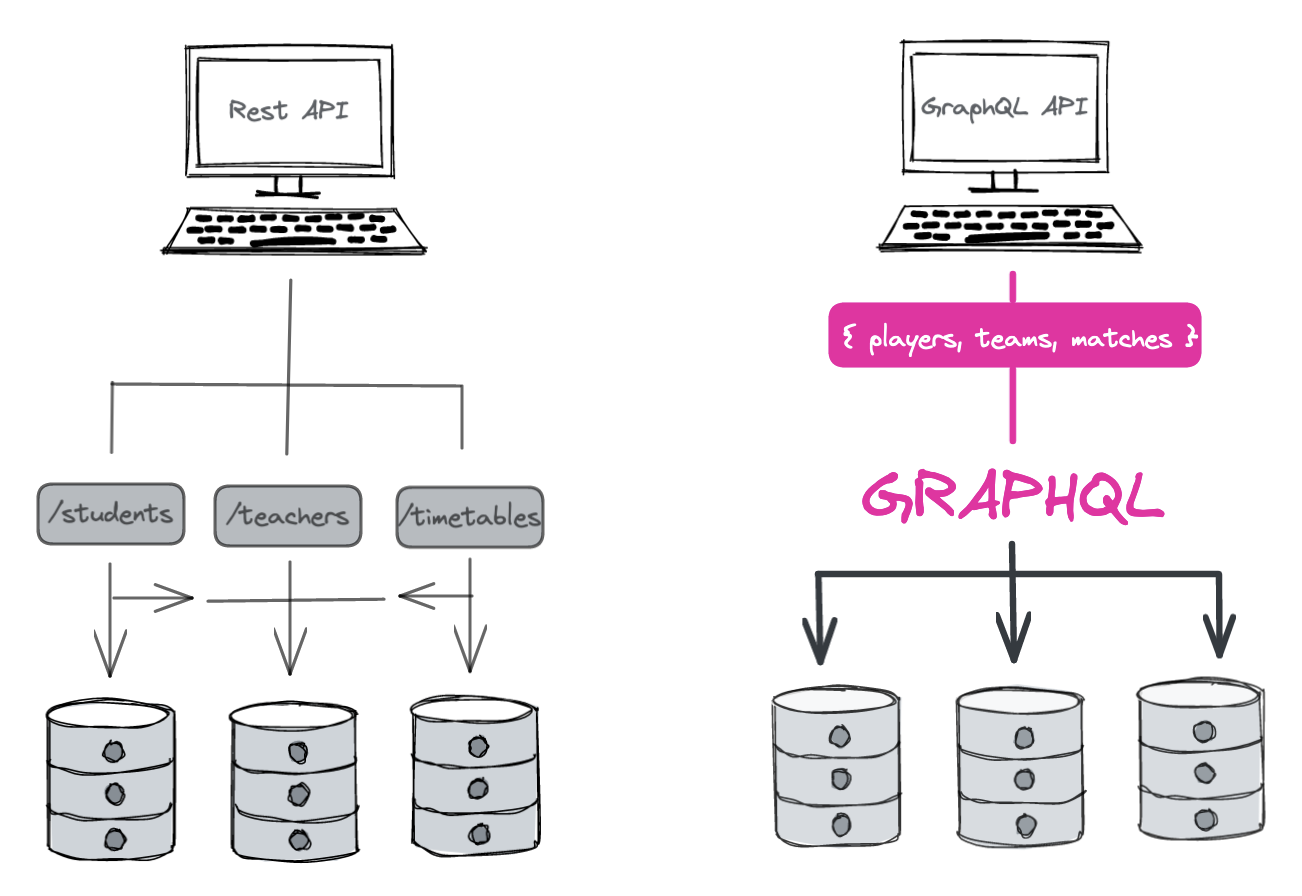
\includegraphics[width=0.7\textwidth]{figures/restvsgraph}
  \caption{Rest API vs GraphQL API}
  \label{f:restvsgraph}
\end{figure}
Querying the API the way users want enables flexibility but can also threaten
security if not appropriately handled. This project aims to enable API producers
to build secure GraphQL APIs without reachable introspection on the endpoint
while still counting on a tool that can generate framework-agnostic structured
documentation.

\section*{Problem Domain}
\label{s:Problem-Domain}
When working on such a problem, there are many different complications as having
updated documentation for GraphQL APIs, one of them - and probably the most
important - being security. Introspection enables users to query a GraphQL API
and discover its schema structure, giving bad actors a chance to discover
potentially malicious operations \citep{khalilWhyYouShould2021} quickly and
disrupt the availability of the API. However, it is also a requirement for tools
such as \textit{GraphiQL} and \textit{Playground}. This is a severe dilemma for
producers who want to keep their APIs as secure as possible, away from
indiscreet eyes, and open to potential threats but still have documentation
tooling. If the attackers have access to the whole schema through introspection,
it will be effortless to find and exploit API calls meant for internal use and
debugging purposes \citep{rizwanGraphQLCommonVulnerabilities2021}. Through the
same technique, the attackers could also get access to mutations and API calls
meant to add, edit or delete specific data on the database, making it a real
threat. Many other security issues are linked to the activation of the
introspection and misconfiguration; some are information disclosure, insecure
direct object references and inexistent ACL \citep{
yeswehackHowExploitGraphQL2021}. By design, GraphQL has a fetching inefficiency
known as \textit{N+1 Problem} where amount of queries executed against the
database (or other upstream services) can be as large as the amount of nodes in
the resulting graph \citep{ graphqlbypopSuppressingProblemGraphQL2020}.
\begin{figure}[H]
  \centering
  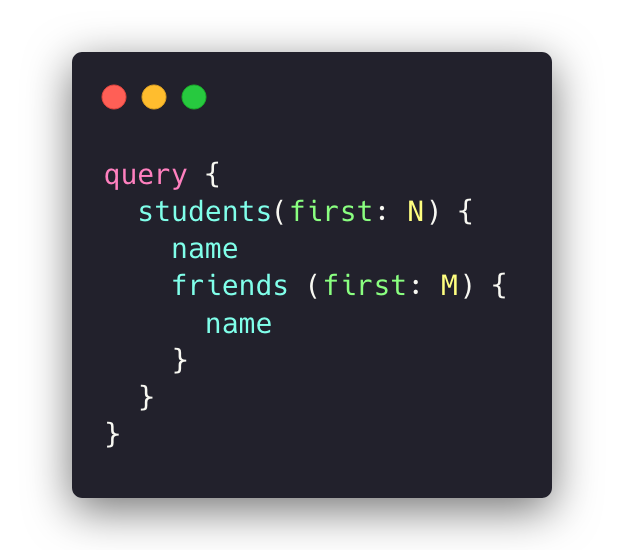
\includegraphics[width=0.5\textwidth]{figures/code/n+1}
  \caption{GraphQL N+1 Problem}
  \label{f:GraphQL-N1-Problem}
\end{figure}
In the example above, the query against the schema would make a single call to
the database to retrieve the first N students, and then for each of these N
students it would make a separate query to the same database to fetch M friends
details (N calls), hence N+1. Having introspection disabled is the right choice
looking at a security perspective, and this project will help solve the downside
of not having tools to help document the API and more.

\section*{Methodology}
\label{s:Methodology}
The project will be divided into two main parts, one being the package to build
the structure and generate the documentation from a single source of truth, in
this case being a GraphQL schema, and the other being the implementation of a
static generated website that renders the previously generated file in HTML
format \citep{gagliardiDjangoRESTMeets2021}. NodeJS will be used as backend
runtime for the backend to generate the documentation that will then be served
to the frontend. The frontend will use NextJS as a React framework to generate
the static HTML files parsing previously generated markdowns. A JAMstack with
Headless CMS approach will be used throughout this project, with additional
content outside the generation scope, being decoupled from the whole versioning
control and being fetched on build time through API queries.
\citep{zammettiWhatJAMstackAll2020}.
\begin{figure}[H]
  \centering
  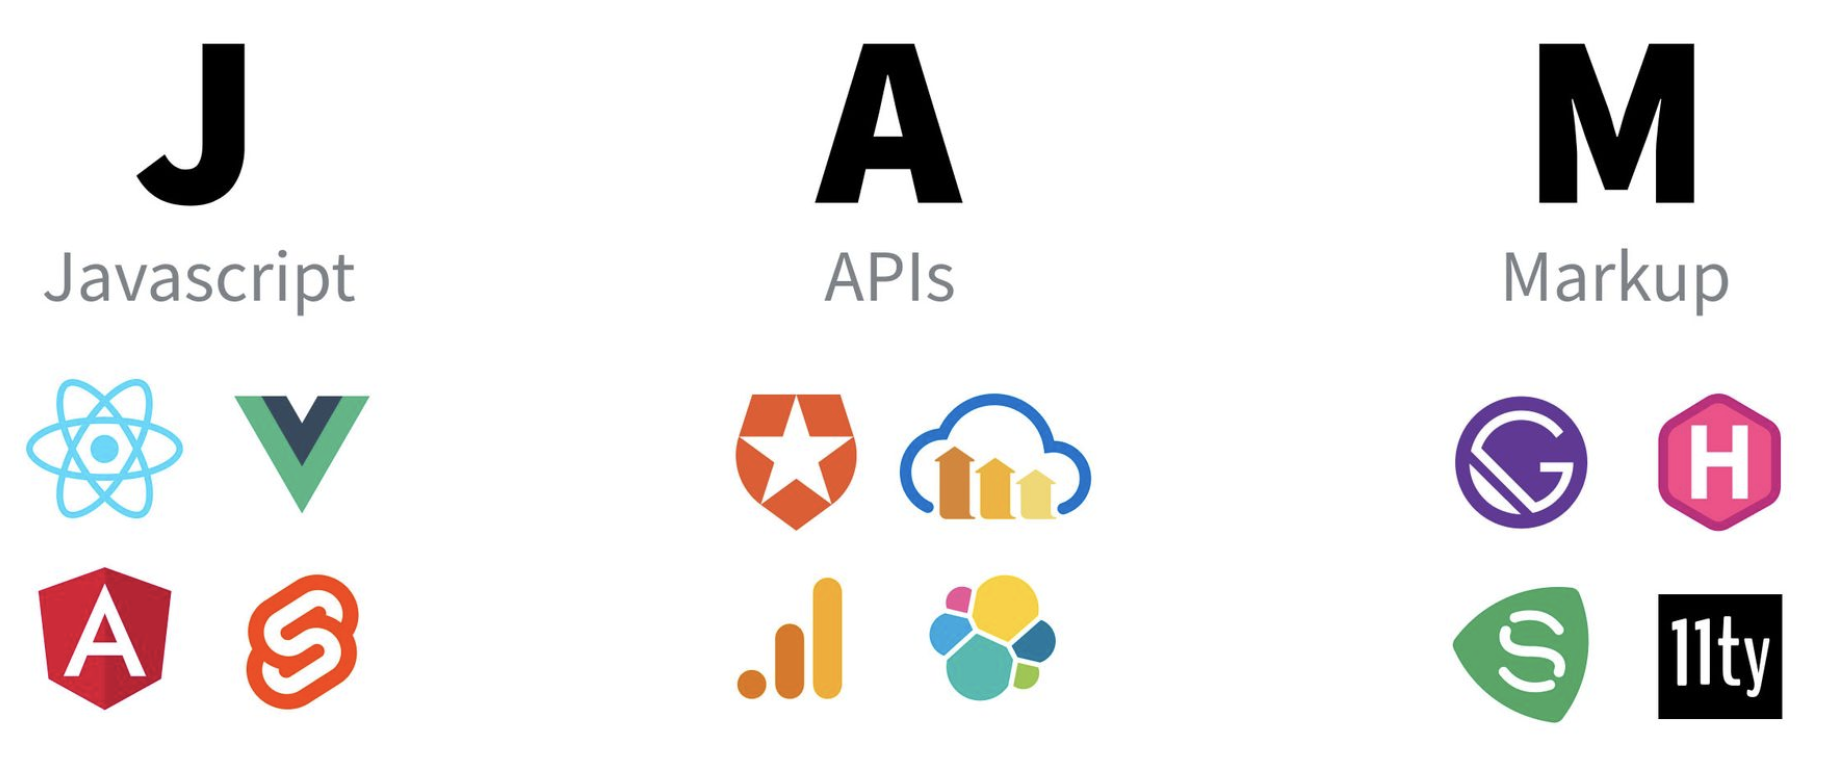
\includegraphics[width=0.5\textwidth]{figures/jamstack}
  \caption{JAMstack breakdown \citep{freecodecampWhatJAMstackHow2020}}
  \label{f:jamstack}
\end{figure}
A Kanban board will be used to maximise efficiency and visualise the workload
and limit the WIP of the project. Kanban has been chosen over Scrum as it is
more flexible and does not require ceremonies to be run daily as standups. Also,
Scrum is overkill for a team of one developer as it would take much time lost on
stories, refinements, pointing, spikes and epics while also managing them over
different sprints \citep{zayatFrameworkStudyAgile2020}. On the other hand,
Kanban will focus much more on delivery and is more suited for a small team or
even an individual developer.
\begin{figure}[H]
  \centering
  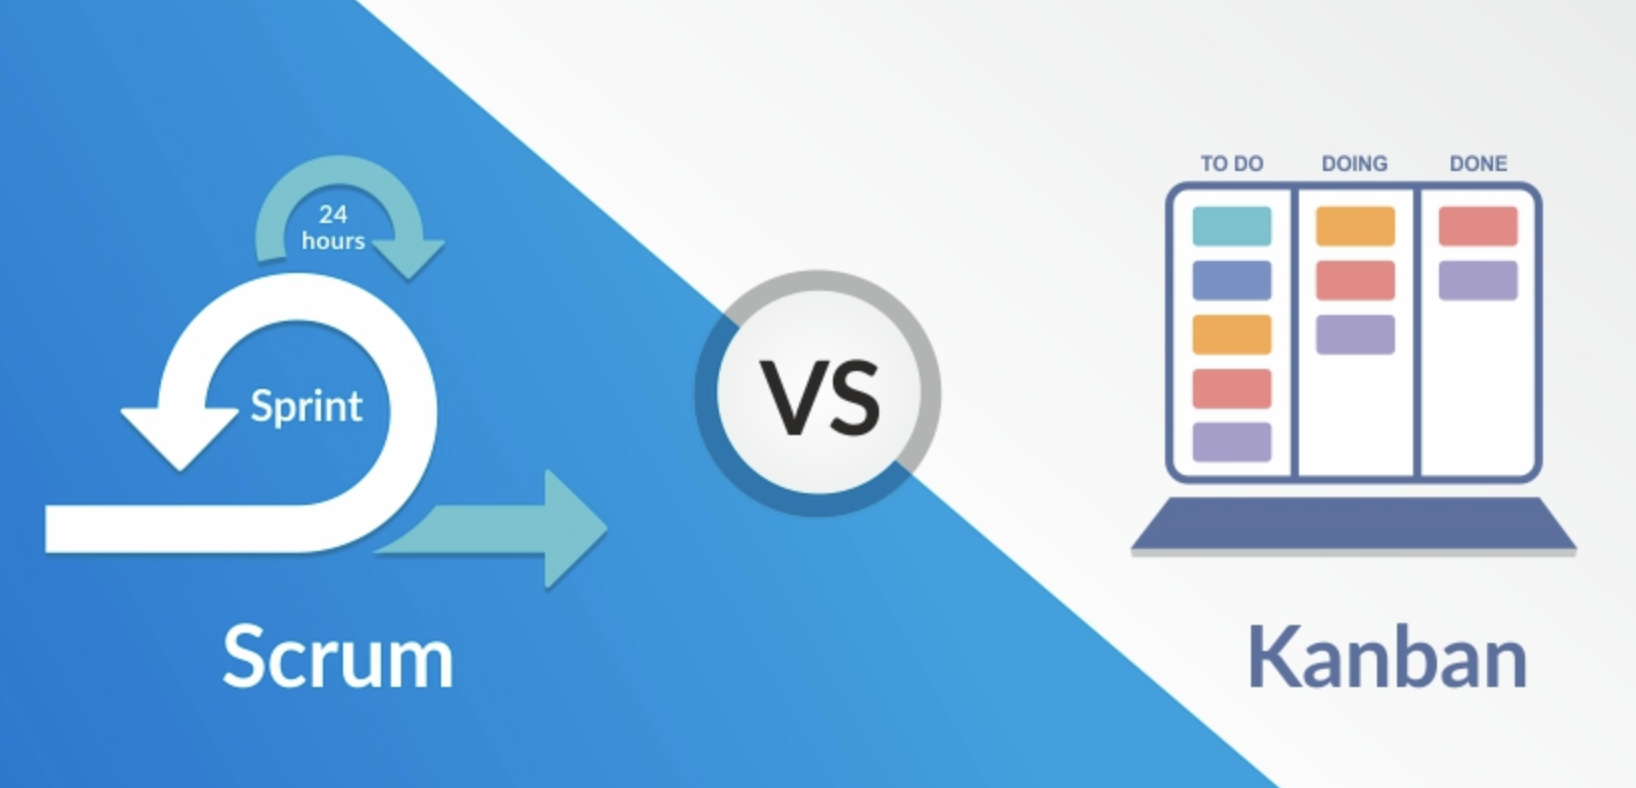
\includegraphics[width=0.5\textwidth]{figures/agile}
  \caption{Scrum vs Kanban \citep{theagilehelpScrumVsKanban2020}}
  \label{f:agile}
\end{figure}
The programming language will be JavaScript for the PoC that will then be
refactored in TypeScript to make the development process more efficient with its
powerful type system saving developer time
\citep{freemanUnderstandingTypeScript2021}. The architecture will be managed
with popular tools such as GitHub for versioning control and single source of
truth for input files, CircleCI for continuous integration, Vercel for
deployment and hosting. To increase package flexibility, the project will also
be containerised building an image through Docker that can run on AWS services
such ECS or EC2 \citep{pratapyadavFormalApproachDocker2021}.

\section*{Evaluation}
\label{s:Evaluation}
A goal-setting methodology will be used to evaluate the project; the initial
goal and key results will be set up at the start of the project with fortnightly
updates. To see if the progress towards the goal is not on the decline, KPIs
will be set to monitor any gaps and focus the attention on the previously set
OKRs. This will help adjust the goals based on the progress and be able to
evaluate if the project reaches a complete state at the end of the deadlines
\citep{helmoldLeanManagementKPI2020}. On the technical side, testing will ensure
that the end product is performant, accessible and meets the expectations set at
the start of the development process. The project will be tested through a
mixture of Unit and E2E tests integrated into the previously stated CircleCI
pipeline before shipping and deploying the code in production environments. This
will ensure that bugged code is only present in non-production environments, and
the last deploy step is reached only when the whole project is ready for
production \citep{yuUtilisingCIEnvironment2020}. The development process will be
evaluated as successful if the OKRs reaches green metrics and the final project
complies with the specifications that have been set
\citep{helmoldLeanManagementKPI2020}. The final product will generate a
structured folder with markdown files that document the references of a GraphQL
schema and being rendered with a JAMstack philosophy.
\begin{figure}[H]
  \centering
  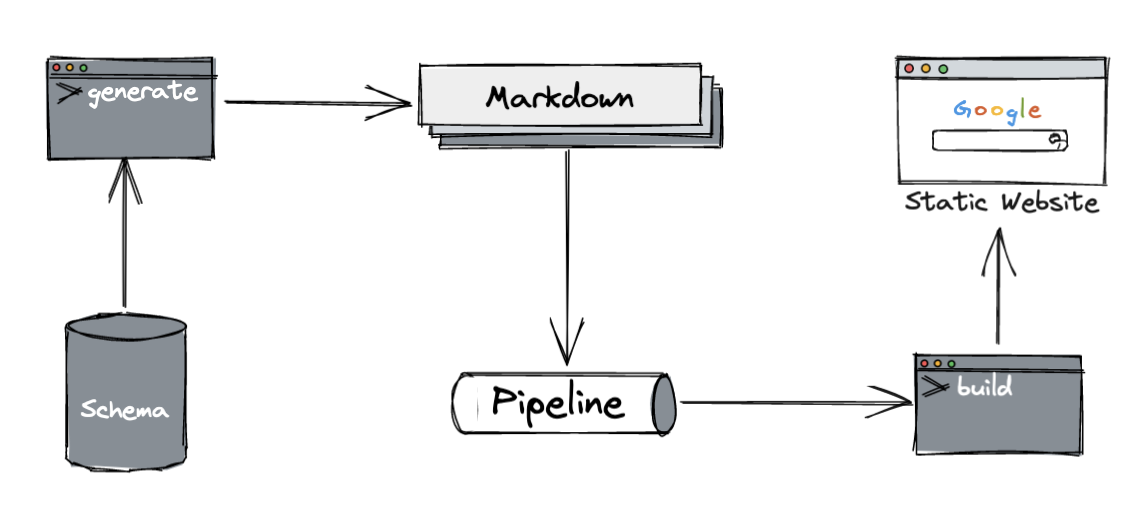
\includegraphics[width=0.7\textwidth]{figures/architecture}
  \caption{High level Architecture}
  \label{f:architecture}
\end{figure}
